\documentclass{article}
\usepackage{graphicx}
\usepackage{amsmath} 
\usepackage{amssymb}
\usepackage{float}
\usepackage{algorithm}
\usepackage{algpseudocode}
\usepackage{subcaption}
%--------- litteratur
\usepackage{natbib}
%---------- 

%---------- hyperref til hyperlink af litteratur
\usepackage[colorlinks=true, linkcolor=blue, citecolor=blue, urlcolor=blue]{hyperref}
%-----------

\title{Bachelor Project 2025}
\author{Johan Søvndahl Kok & Conrad Lavesen Valentinus}
\date{February 2025}
% --------- Fodnoter og litteratur ------

% -------- fodnoter og litteratur -------

\begin{document}
\maketitle
\newpage
\tableofcontents
\newpage

\section{Abstract}


\section{Introduction}

\section{Economic Theory}
HAL R. Varian "Intermediate Microeconomics with calculus"
\newline 
The “Cournot-Bertrand Debate”:
A Historical Perspective 
https://competitionandappropriation.econ.ucla.edu/wp-content/uploads/sites/95/2020/12/CournotBertrand-debate.pdf
Jean Magnan de Bornier 
\newline
Steven Tadelis--- Game theory -  An introduction.
\newline
In the following section we will focus on unraveling the Economic theory behind the dynamics of the game we will be simulating. 

We will be setting the simulation up like a Bertrand economy as in the works of Maskin and Tirole.

General game theory will be introduced based on the works of (......).

In regards to the economic constraints forming the demand functions, we have chosen the following: (-..-....). The economic constraints we have chosen are based on the works (......).

We simulated the game using different strategies. The strategies we ended up choosing were tit for tat (known from the work ....) and different forms of Q-learning (from .........)


We are investigating the dynamics of the game and specifically what happens when you change the number of prices that each firm can set (we call that parameter k).


\subsection {Game Theory}
\label{GameTheory}
Game theory, broadly speaking, is a way to provide a framework for trying to understand how rational agents make decisions in individual and group settings, when agents' payoffs depend on their own and other choices. It has been applied in a lot of fields, also outside of economy such as biology. In relevance, to our project, it has been used successfully in competitive areas such as business competition. (TADELIS)
\newline
The framework of the simulations in our project are based on game theory. Therefore, we will now introduce project-relevant definitions from game theory and assumptions which will be used when setting up our simulations.
\newline
First off, agents (or players), will be referred to as firms, and are assumed to be rational, meaning that they act according to the actions which maximizes their payoff (TADELIS). In regards to our project, this means that the firms' objective is to maximizing profits.
\newline
Firms can choose to set different prices when playing against each other. Thus, setting prices are the actions that the firms can take.
These prices are 'strategies', when we analyze the setting from a game theory perspective. 

With these strategies, we can end up with different equilibria.
\subsubsection{Nash Equilibrium, SPNE and MPE}
A \textbf{Nash equilibrium} is a strategy or set of strategies in a game where no agent  has any incentive to deviate from their strategy, given what the other agents are playing (Tadelis).
\newline
In our simulation we are playing a repeated game, which leads us to the definition of the Subgame Perfect Nash Equilibrium (SPNE). A SPNE is a refinement of the Nash equilibrium and means that every subgame of the game is a Nash equilibrium \cite{tadelis} (page 157). 
\newline
A Markov-perfect equilibrium (MPE) is a term introduced by \cite{MaskinTirole} which is a subgame perfect Nash equilibrium under the Markov assumption. The Markov assumption is that only directly relevant payoffs are used to determine the strategy of the firms. This means that e.g. the history of the prices are irrelevant, other than the price the competing firm set in the last period, $p_{j,t-1}$. 
\newline
Edgdeworth price cycles (eventuelt) and focal pricing




\subsection{Bertrand competition}
The overall competition framework used in the project, will be based on the ideas of Joseph Louis François Bertrand. In a market for a homogeneous good, sold by symmetric firms, Bertrand came up with the theory, that the firms will only be setting the price while the market then will be determining the quantity sold(VARIAN). Bertrand's logic can be used on oligopolies, but as Bertrand originally framed his arguments in 1883 (Jean Magnan De Bornier), this project will be in the setting where only 2 firms exist on the market, namely duopoly. 
\newline
The reasoning for choosing our setting as a duopoly follows from the settings of \cite{MaskinTirole} and \cite{Klein2021},
where we are using the same base for our model. They both model the pricing competition using a setting with two firms. The ideas of price cycles such as Edgeworth cycles or the dynamics of focal pricing, are described for two firms. Therefore, it is sensible that our setting is also based on two firms, such that we can analyze the dynamics that arises from our model.
Furthermore, we are investigating the dynamics of what happens when we change the number of price points, meaning the number of different prices that the firms can set (referred to as the parameter k). It is therefore computationally heavy when you introduce more than two firms in the simulation, as the computations needed to be done rises with the parameter \textit{k}.  
\newline
Bertrand originally showed that under all the assumptions above and an assumption of constant cost, the Bertrand equilibrium is when the price is equal to the marginal cost, which is also a Nash equilibrium. However, in markets with few sellers, firms do not typically sell their goods at the marginal cost. 
\cite{MaskinTirole} partly blame this on the fact that the original model proposed by Bertrand was static, meaning that both firms set their prices simultaneously without knowing what the other firm set as a price, and the market clears and the game ends. They argue that having a dynamic model may be important to capture the dynamics of actual price competition. \cite{MaskinTirole}
In a dynamic model, firms set prices in multiple rounds. This is important for us, as we are investigating the dynamics of price competition.  
\newline
Furthermore, our dynamic model is sequential, meaning that firms take turns setting their prices. \cite{Klein2021} argues that a sequential dynamic model is a more realistic model to capture pricing competition from the real world.
Other researchers, such as \cite{Calvano} have used a simultaneous dynamic setting, where firms play a repeated game, but set their prices in each turn at the same time. We believe that the sequential dynamic setting used in \cite{Klein2021} is more representative of the real world, as it is unlikely that firms always would set prices on the same goods, at exactly the same time. In a duopoly setting, it is more realistic that one firm sets a price, then the second firm observes that price and sets their price, and then the first firm sets their new price based on the price from the second firm. 


\subsection{Economic environment}

We will be looking at a sequential pricing duopoly as in \cite{Klein2021}. In the model, firms set prices sequentially, meaning they take turns on setting prices. The model uses Q-learning in a simulation setting, which we will also do.
We will now further describe the economic environment, which is based on the work of \cite{Klein2021}. 
\newline
Two firms, \textit{i} and \textit{j} take turns on setting prices in infinitely repeated discrete time indexed by $t = \{1,2,3,... \} $. Thus, firm \textit{i} sets price $p_{i,t}$ and firm \textit{j} sets the price $p_{j,t}$ in period \textit{t}. 
The prices that the firms can choose are discrete, evenly spaced and between 0 and 1. The number of different prices that the firms can set are determined by \textit{k}, such that the price interval is denoted by $P = \{0, \frac{1}{k}, \frac{2}{k}, \frac{3}{k},...,1\} $. Prices are set sequentially, such that in even time periods firm $p_i$ sets their price, and in odd time periods $p_j$ sets their price.
\newline
Assuming no marginal or fixed costs, the profit function for firm \textit{i}, in time period \textit{t} is described as:
\begin{equation}
    \pi_i (p_{it},p_{jt}) = p_{it}D_{it}(p_{it},p_{jt})
\end{equation}
where $p_{jt}$ is the price of the opposite firm, and $D_{it}$ is the demand as a function of its own price $p_{it}$, and the price of the opposing firm, $p_{jt}$.
\newline
-------------------
Firms discount future profits with $\delta \in [0,1)$
-------------------
\newline
The demand function is defined as:
\begin{equation}
D_i(p_{it},p_{jt}) =
\begin{cases}
  1-p_{it} &\text{if } p_{it} < p_{ij},\\
  \frac{1-p_{ij}}{2}   & \text{if } p_{it} =p_{ij},\\
  0   & \text{if } p_{it} > p_{ij}
\end{cases}
\end{equation}
Where the firm with the lower price takes the whole market. In the case where they set the same price, they share the market. The monopolist's price is the same as the collusive joint-profit maximizing price. Therefore, we calculate the monopolist's price, such that it can later be used as a benchmark and visualization of when the firms are setting supra competitive prices. Meaning prices that are above the competitive benchmark, which we will return to in SECTION ?!?!?.
\newline
The monopolist's demand function is:
\begin{equation}
    D(p) = 1-p
\end{equation}
with a profit of
\begin{equation}
    \pi (p) = p \cdot D(p) = p \cdot (1-p) \Leftrightarrow \pi (p) = p - p^2
\end{equation}
maximizing over p, we take the derivate with respect to p: 
\begin{equation}
    \cfrac{d \pi(p) }{d p} = 1-2p
\end{equation}
and now setting the equation equal to 0 and isolate for p:
\begin{equation}
    0 = 1 - 2p \Leftrightarrow p = \cfrac{1}{2}
\end{equation}
Which means that the joint-profit maximizing price is:
\begin{equation}
    p^M = 0.5
\end{equation}
with a profit for each firm of:
\begin{equation}
\pi_{ij}^M (p^M) = 0.5 \cdot \cfrac{1 - 0.5}{2} = 0.125
\end{equation}
-------------------------------
Which will serve as our benchmark for tacit collusion in this project.  
-------------------------------
\label{Joint_profit_price}
\newline
Following the works of \cite{Klein2021} and \cite{MaskinTirole}, we impose the Markov assumption: only directly relevant payoffs are used to determine the strategy of the firms. This means that the strategy that the firms follow, are only dependent on the price that the other firm set in the last period $p_{j,t-1}$. This implies that the history of the prices (other than the last period) are irrelevant, and that there is no communication between the firms.
Here, strategies are the prices that the firms are setting.
\newline
Because we are in a dynamic environment, we will define what will be an equilibrium in this setting. 
The following value function is a Nash equilibrium for all prices along the equilibrium path, if the condition holds for both firms:
\begin{equation} \label{KleinBellmanEq}
    V_i(p_{jt}) = \mathop{\text{max}}_{\textbf{p}} [\pi_i (p,p_{jt}) + E_{p_{j,t+1}}[\delta \pi_i (p,p_{j,t+1})+\delta^2 V_i (p_{j,t+1}) ]]
\end{equation}
Where $\delta$ is a discount factor, discounting how much firms value future profits. Where a discount factor of 0 means that firms do not care about future profits at all, while a discount factor closer to 1 means that the firms almost value future profits as much as current profits. 
Equation (\ref{KleinBellmanEq}) is written in the style of \cite{Klein2021}, who has the equation from \cite{MaskinTirole}. They introduce the concept of Markov Perfect Equilibria (MPE) and if you include off-equilibrium prices, for all prices a strategy pair $(R_1,R_2)$ is MPE if the above equation holds.
\newline
--------Nash equilibria one increment above the lowest price? Mentioned in Klein. Mentioned by Anders.----------------
\newline

\subsubsection{Edgeworth Price Cycles and Focal Pricing} \label{EdgeworthFocalpricingSec}
Further, \cite{MaskinTirole} show that if firms value future profits sufficiently \footnote{When \cite{MaskinTirole} talk about valuing future profits 'sufficiently' high with a 'sufficiently' high discount factor, they mention one close to 1, without giving a specific number. An idea of a sufficiently high discount factor is calculated to be ??0.877?? in the works of KILDE?!?!??!?!??!}, two kinds of MPE's exist, 
namely focal pricing and Edgeworth price cycles.
Focal pricing is when both firms are playing the same price, repeatedly. This equilibria exists because of the fear from the firms, that if they undercut their competitor, that the competitor would follow suit and undercut them aswell. This would start a price war, which would be costly for the firms. And because they value future profit sufficiently, none of the firms are willing to start this price war. Similarly, the firms are not willing to increase the price, as they believe that the other firm would not follow, and then they would lose the entire market.
\newline
Edgeworth price cycles are when firms gradually undercut each other, to increase market share, until the price war becomes too costly (price reaches marginal cost, which in our case is 0), and one of the firms resets the price to a 'high' price (one increment above the monopoly price), and the undercutting begins again (\cite{MaskinTirole}). In this way, a cycle pattern arises, which can be seen in Figure \ref{fig:EdgeworthCycle}.

\begin{figure}[H]
    \centering
    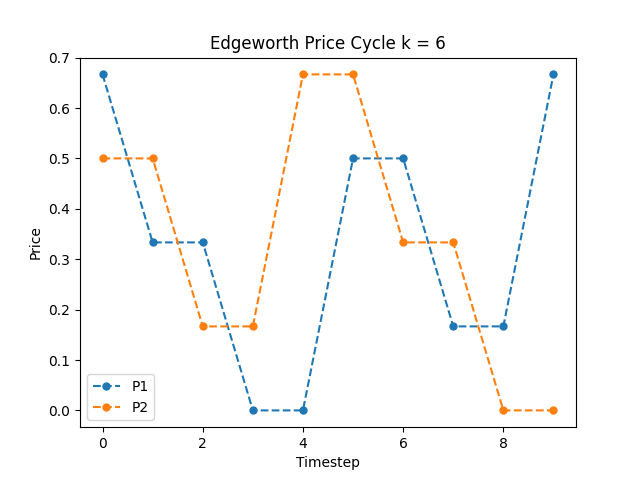
\includegraphics[scale = 0.75]{Edgeworth price cycle k = 6.png}
    \caption{Edgeworth price cycle for two firms with k = 6. Firms undercut each other until the first firm to observe the lowest price resets the price cycle. In this case firm 2 are the first to reset the cycle, and then the next reset is done by firm 1.}
    \label{fig:EdgeworthCycle}
\end{figure}
The Edgeworth price cycle changes, as the price interval changes (number of prices that the firms can set, denoted by parameter \textit{k}). This is important to note, as we will later analyze what happens when \textit{k} changes. 
\newline
We simulate the Edgeworth cycles with different values for \textit{k} in Python, and calculate the per period profit corresponding to the Edgeworth cycle with a given \textit{k}.
The per period profit of the Edgeworth price cycle will serve as a benchmark for the competitive level of profit, just as it does in \cite{Klein2021}. For $k = 6$, the per period profit is $\pi = 0.0611$. Note that other candidates for the competetive benchmark are the static Nash outcome of the game where both firms set the price at the marginal cost (or one increment above the marginal cost), both of which is a static Nash equilibrium. However, due to the dynamics of the game, the static Nash outcome is not a suitable benchmark for a repeated game (\cite{Klein2021}).
\newline
As we are investigating what happens when \textit{k} changes, we need to calculate the per period profit of the Edgeworth cycles. This is done using our Python script and the results are reported in table (\ref{tab:kPrPeriodProf})

\begin{table}[H]
    \centering
    \begin{tabular}{|c|c|}
        \hline
        Size of price interval, \textit{k} & Per period profit of the Edgeworth cycle \\
        \hline
        k = 6 & 0.0611 \\
        \hline
        k = 12 & 0.0699 \\
        \hline 
        k = 24 & 0.0758 \\
        \hline
        k = 48 & 0.0793 \\
        \hline
        k = 100 & 0.0813 \\
        \hline
    \end{tabular}
    \caption{The per period profit associated with the Edgeworth price cycle for different values of \textit{k}.}
    \label{tab:kPrPeriodProf}
\end{table}




\section{Reinforcement learning theory} \label{ReinforcementLearningTheory}

\subsection{Introduction to Reinforcement Learning}
Reinforcement learning (RL) is a concept from machine learning, that differs from other types such as supervised learning and unsupervised learning.
Supervised learning is where you have labeled input-output pairs, and the objective is then to find the unknown function which this data is from. An example of supervised learning could be the very well-known OLS regression which tries to fit a linear model to data. In unsupervised learning, you have access to unlabeled data, and the objective is to find patterns or structures. An example of unsupervised learning could be K-means clustering which tries to find clusters in unlabbeled data, thereby finding the patterns. RL differs from these methods, and instead learns the most optimal choices through repeated interactions with the environment. This is therefore a 'trial and error' approach, where the algorithm tries new actions, and learns through which actions give the best rewards. A great and relevant example of an RL algorithm would be Q-learning (MARL side 19-21). 
\newline 
\newline
A more general definition of RL is provided in the book "Multi-Agent Reinforcement Learning:
Foundations and Modern Approaches" by Stefano V. Albrecht,  Filippos Christianos,  Lukas Schäfer, which will also serve as a primary source of this theory section and subsections. The defintion: 
"\textbf{Reinforcement learning (RL) algorithms learn solutions for sequential
decision processes via repeated interaction with an environment.}"
The following explanations are of the sentences populating the definition.
\textbf{Learning via repeated interaction:} "Finally, RL algorithms learn such optimal policies by trying different actions in different states and observing the outcomes."
Learning via repeated interactions is thereby where RL gets its "trial and error" understanding.
\textbf{Sequential decision process:
}"A sequential decision process is defined by an agent that makes decisions
over multiple time steps within an environment to achieve a specified goal" 
\textbf{Solutions:}"A solution to the decision process is an optimal decision policy for the agent,
which chooses actions in each state to achieve some specified learning objective." 
\newline
(MARL side 20)
\newline
\newline
To define Sequential Decision processes, we would need to define a decision process model from which these decisions can be made and in order to find a solution (an optimal strategy), we would need to define a learning objective to evaluate each strategy. Together, the decision process model and the learning objective form a reinforcement learning problem, which is illustrated in Figure \ref{fig:MARLside20} (MARLside20). The decision Process Model we will be using, in relation to our implementation of Q-learning, will be the Markov Decision Processes, which will be referred to as MDP for short.
\newline 
\newline
The environments in which we implement our RL algorithms determine whether we are dealing with Multi-Agent RL or Single-Agent RL. The two concepts of Single and Multi-agent RL will be elaborated upon later, but two quickly summarize: Single-agent RL interacts with an environment alone, while  Multi-agent acts with an environment with other agents. (MARL SIDE 19-21).
In this section, we will unpack the theory essential to understanding the underlying principles of Q-learning, beginning with the single-agent framework and MDP, trying to translate the general Q-learner setup to our Economic environment. 
\begin{figure}
    \centering
    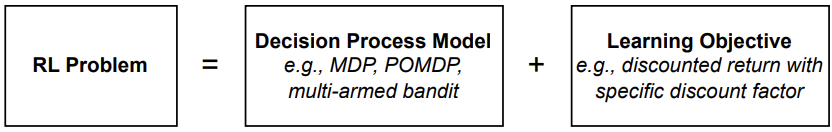
\includegraphics[width=0.5\linewidth]{MARLside20.png}
    \caption{Figure from MARL side 20 }
    \label{fig:MARLside20}
\end{figure}
\subsection{Single Agent RL}
In this subsection we will be attacking the theory of RL in the Single-agent approach, many of the following concepts that will be introducet  lay the groundworks .... NOTE Menation that this subsection is based in a single anget approach etc....
\subsubsection{Sequential decision process}
As hinted earlier, Markov Decision Processes (MDP) will be the Decision Process Model that we will focus on. It serves as the standard model for sequential decision processes that lays the foundation for
defining single-agent decision processes in RL (MARL side 19-22). This can be set in more intuitive terms: MDP provides a structured way to model the process where an agent must make a series of decisions over time in an environment.
\newline
\textbf{(Definition: Markov Decision Process) MARL SIDE 22} A Discrete (MDP) consists of:
\begin{enumerate}
    \item \textbf{Finite set of states \( S \)}, with a subset of terminal states \( \bar{S} \subset S \).
    \item \textbf{Finite set of actions \( A \)}.
    \item \textbf{Reward function \( \mathcal{R}: S \times A \times S \to \mathbb{R} \)}.
    \item \textbf{State transition probability function \( \mathcal{T}: S \times A \times S \to [0, 1] \)} such that
    \[
    \forall s \in S, a \in A : \sum_{s' \in S} T(s, a, s') = 1 \quad 
    \]
    \item \textbf{Initial state distribution \( \mu: S \to [0, 1] \)} such that
    \[
    \sum_{s \in S} \mu(s) = 1 \quad \text{and} \quad \forall s \in \bar{S}, \mu(s) = 0 \quad 
    \]
\end{enumerate}
Let us now try to explain exactly what this mean starting with the first item of the definition.
b\newline 
\textbf{Finite set of state S}  are the possible situations that an agent could be in, this could be a current competitor price for a company. Terminal states are also allowed to be substituted for by a maximum number of time steps, to ensure termination. 
\textbf{Finite set of actions A} set of actions A are the possible actions that an agent would have. For example, the amount of different prices an agent can set. 
The \textbf{Reward function} determine the reward of an action and thereby how well the action was guiding the agent. It could be a profit function that takes a price, thereby an action, as inputs. The \textbf{State Transition function's} goal is to explain explains how the environment changes when the agent. It can be fought of like a rulebook, containing rules of the game. This could be the rules that clearly illustrates what happens when be a firm sets a price. 
The \textbf{Initial State Distribution} defines the probabilities of starting in each possible state when the environment begins, and the agent starts its learning journey. It tells us the chances of the agent being in a particular state at the beginning. For example, if a firm has two possible starting states $s_1$ and $s_2$ the initial state distribution might look like $s_1=30\%$ and $s_2 = 70\%$ meaning there's a $30\%$ chance the firm starts in state $s_1$ and a $70\%$ chance it starts in state $s_2$.
\newline 
\newline 
One could easily think that the Markow Decision process could have something to do with the Markow assumption, also known as the Markow property mentioned in section \ref{GameTheory}, and indeed it does. 
As we know, the Markow assumptions states that the future state and reward conditionally independent of past states and actions, when you have the current state and action. Mathematically the assumption is expressed in equation \ref{Markow_property}.
\begin{equation}
\label{Markow_property}
P(s_{t+1}, r_t | s_t, a_t, s_{t-1},a_{t-1} \dots, s_0, a_0) = P(s_{t+1}, r_t | s_t, a_t)
\end{equation}
(MARL side 23)
This allows us to only give an agent the current state and it would still be sufficient information for it to take optimal actions in an MDP. The assumption allows us to even further limit or "spare" and have it be unbeknownst to our reward and transition functions, as the current state is sufficient information. The agent will also know the state space and action space.  (MARL side 23)
Limiting the agent therefore limits the amount of complex coding and makes the process less computationally demanding, by not needing to store and use past states and actions.  
\subsubsection{Value functions and Bellman equation}

\subsubsection{Temporal difference Learning and Q-learning}
Exploration vs. Exploitation
AND 
Epsilon-Greedy Method and MAYBE CONVERGENCE


\subsection{Multi Agent RL}
Now that the section above have given a better understanding of the theory and methods behind how single agent RL works, we will now move onto multi agent reinforcement learning. The relevance of both having multi agent and single agent RL theory and methods will become clear in the following. Figure \ref{fig:marside44} from MARL side 44 finely illustrates an overview of the Multi-agent RL Hierarchy. It illustrates how Repeated Normal-Form games and Markow Decision Processes are special cases of Stochastic Games which are special cases of Partially Observable Stochastic Games. The figure also shows what number of states and agent classify each type of game. In this thesis we are focusing on Q-learning and Q-learners (agents) playing and learning against each other. The states will be fully observed and transparent for each agent and combining it with having multiple agents working in the same environment means we only will be exploring the Stochastic games and Markow decision processes.
\begin{figure}[H]
    \centering
    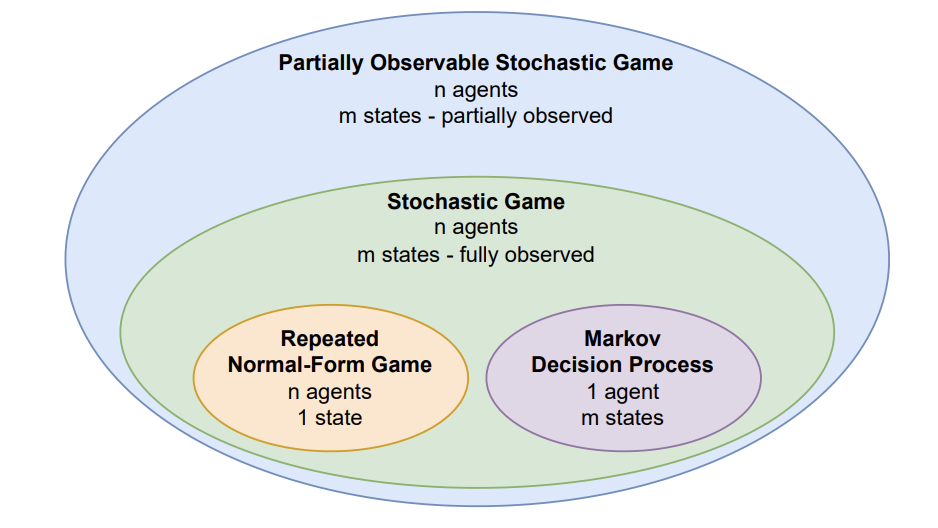
\includegraphics[width=0.5\linewidth]{Multi-agent-figure.png}
    \caption{Figure from MARL side 44 }
    \label{fig:marside44}
\end{figure}
\subsubsection{Stochastic games and Independent Learning}
Most of the theory that Stochastic games are build upon is very similar to MDP's and therefore to avoid repeating ourselves the following will seem more superficial. A more formal definition of a stochastic game is given in definition 3 from MARL side 47-48. 
\newline
\textbf{Definition 3 (Stochastic game)} A stochastic game consists of:
\begin{enumerate}
    \item Finite set of agents \( I = \{1, \dots, n\} \)
    \item Finite set of states \( S \), with a subset of terminal states \( \bar{S} \subset S \)
    \item For each agent \( i \in I \):
    \begin{itemize}
        \item Finite set of actions \( A_i \)
        \item Reward function \( R_i: S \times A \times S \to \mathbb{R} \), where \( A = A_1 \times \dots \times A_n \)
    \end{itemize}
    \item State transition probability function \( T: S \times A \times S \to [0, 1] \) such that
    \[
    \forall s \in S, a \in A : \sum_{s' \in S} T(s, a, s') = 1
    \]
    \item Initial state distribution \( \mu: S \to [0, 1] \) such that
    \[
    \sum_{s \in S} \mu(s) = 1 \quad \text{and} \quad \forall s \in \bar{S}: \mu(s) = 0
    \]
\end{enumerate}

From the definition it is clear to see that it is just an expansion of the definition for the MDP and making it able to handle multiple agent in the same environment. Similar to the MDP, the Stochastic games have the same Markow Assumption as shown in equation \ref{Markow_property}. All these similarities, making it no wonder why Stochastic Games are also referred to as Markow Games MARL side 48.
\newline 
\newline
Multi-agent reinforcement learning can be used to learn strategies for handling real-world problems. And since the problems that RL are used to solve differs quite a bit, the approach on to actually apply the RL also differs quite bit. In this thesis, we will be using the approach of reducing 
a multi-agent RL game into multiple single-agent RL games within the Multi-agent game. This is standard approach in RL which lowers complexity by reducing the multi-agent learning problem to a single-agent learning problem. More specifically there are 2 different ways to execute this approach, respectively, Central Learning and Independent Learning. Central Learning is when you take the joint action space for multiple agents and then apply single Agent RL to the joint actions actions space all together, therefore learning a central strategy that chooses actions for all agents. Central Learning could therefore make sense to use in environments where the agents work together. Independent Learning is when you apply single agent RL to each agent independently, essentially isolation each agent. This means that each agent learns their own independent strategies and ignore the presence of the other agents. They just see the agents as part of the environment. Independent learning would there be a great approach for environments where agents work against each, which is why this is the approach we have been using in the thesis (Side 95 MARL). 
\newline
\newline
........ The independent Learning approach to multi-agent Reinforcement Learning bring us to Q-learning algorithm number 2 (MARL side 98), which is easy to recognize, as it is just an expansion of Algorithm 1  
\newline
\newline 
\begin{algorithm}
\caption{Independent Q-learning (IQL) for stochastic games}
\textbf{Algorithm controls agent \(i\)}
\begin{algorithmic}[1]
\State Initialize: \( Q_i(s, a_i) = 0 \) for all \( s \in S, a_i \in A_i \)
\State Repeat for every episode:
\For{$t = 0, 1, 2, \dots$}
    \State Observe current state \( s^t \)
    \State With probability \( \epsilon \): choose random action \( a_i^t \in A_i \)
    \State Otherwise: choose action \( a_i^t \in \arg \max_{a_i} Q_i(s^t, a_i) \)
    \State (meanwhile, other agents \( j \neq i \) choose their actions \( a_j^t \))
    \State Observe own reward \( r_i^t \) and next state \( s^{t+1} \)
    \State \( Q_i(s^t, a_i^t) \gets Q_i(s^t, a_i^t) + \alpha [r_i^t + \gamma \max_{a_i} Q_i(s^{t+1}, a_i) - Q_i(s^t, a_i^t)] \)
\EndFor
\end{algorithmic}
\end{algorithm}




nederst sektion side 89
Convergence Our game  is it possible or what etc. 

\subsection{Linking everything to Economic, maybe should just do that along the way ? probably better}
Algorithm 5 page 98





\section{Setup for simulation}

In this section we will describe how we are running the simulation, and what parameters are being used. 

When running the simulations, we are letting two Q-learners compete against each other, as in the theoretical frame that we set up earlier.

The setup for the simulation is following the work of \cite{Klein2021}. This is done such that results are comparable.
We are running the simulations over $500,000$ timesteps (T=500,000), and then doing that a $1000$ times. In the graphs, the average is a running average taken over $1000$ timesteps each time. This is to smooth out short term fluctuations, where the algorithms are learning, and trying out setting new prices. The average profit in the end is reported as the average profit in the last $1000$ rounds. This is because we are interested to see what level of profit the Q-learning algorithms are making when the algorithms have 'converged'. In the end of the simulation the algorithms have converged (KAN gøre some Calvano et. al og sige det er konvergeret når den gennemsnitlige profit er den samme i x antal perioder).
Klein side 547 Collsuive equlibria. Vi ser det som collusion når profit er over kompetitivt benchmark bla bla bla.

\subsection{Parameters}
As described in section \ref{ReinforcementLearningTheory}, there are different values that can be chosen for the parameters. We need values for $\delta$, $\alpha$, $\theta$, $\epsilon_t$ and \textit{k}. All of these parameters can undertake different values, and in this section we will justify our choices.
\newline
The discount factor, $\delta$, corresponding to how much the firms value future profits, is chosen to be: 
$$\delta = 0.95$$
The discount factor needs to be large enough for the firms to care enough about future profits, such that it is even possible for the algorithms to get collaboration/collusion going. Time periods are generally small, which justifies a discount factor close to one. \cite{Klein2021} found the optimal discount factor to be $0.95$, and it is also the same discount factor that is being used in \cite{Calvano}, and thus we will also use it.
\newline
The learning rate, $\alpha$, determines how much new information is weighed relative to existing knowledge. It should be high enough to incorporate new insights, but not so high that it causes the Q-learner to forget what it has already learned. Through simulations \cite{Klein2021} has found the optimal learning rate to be:
$$\alpha = 0.3$$
Which is also the one we will be using.
\newline
If we recall the $\epsilon_t$ it determine the probability of a Q-learner chosing a random action instead of a calculated one given a time step t, therefore calling it the exploration parameter. It is determined by the following equation:
\begin{equation}
\label{eq:epsilon-theta}
    \epsilon_t = (1-\theta)^t 
\end{equation}
Equation \ref{eq:epsilon-theta} makes it such that the algorithm will do a lot of exploration in the beginning, and then gradually decrease. Equation \ref{eq:epsilon-theta} illustrates why $\theta$ is called the decay parameter, as a larger $\theta$ value will make the decay of the exploration parameter happen faster. As in \cite{Klein2021}
$\theta$, the decay parameter, is chosen such that at $\epsilon_0 =100\%$,  $\epsilon_{250,000} =0.1\%$ , $\epsilon_T = \epsilon_{500,000}=0,0001\%$. This means that a $\theta=0.0000275$ as this will equal to: \begin{equation}
    \epsilon_{500,000}= (1-0.0000275)^{500,000}=0.0000010675\approx 0.0001\%
\end{equation} 


\subsection{Evaluating performance}
We need to evaluate the performance of the Q-learning algorithm, and have benchmarks that will help us in understanding the results. 
As mentioned earlier in section \ref{EdgeworthFocalpricingSec}, we use the average per period most profitable Edgeworth cycle as the competitive benchmark. The per period profits for some values of \textit{k} can be seen in table \ref{tab:kPrPeriodProf}. As mentioned in section \ref{Joint_profit_price}, we will be using the joint-profit maximizing profit as a collusive benchmark. 
\newline
To determine what strategies and thereby any cycles a 2 agent Q-learning game has converged to we have come up with the following. We check the last 1000 time steps, given us a  $\epsilon$ value of:
\begin{equation}
    \epsilon_{499,000}= (1-0.0000275)^{499,000}=0.000001097267\approx 0.000109\%
\end{equation} 
This means that at timestep $t = 499,000$, there is a $0.000109\%$ chance for the algorithm to explore and thus try something randomly new. 
We believe that such an epsilon value is sufficient for assuming that no further exploration takes place for either of the Q-learners and the Q-learners has thereby converged to some strategies, whether these are focal pricing or cycles. Another worry could be the length of potential cycles exceeding a length of the 1000 and it would thereby slip through our monitoring. As we will see later this will not become an issue, as the length of cycles rarely exceed 40 steps and even when k=100. 

\section{Results}
\label{Results section}
The following section has been divided into 3 subsections. \textbf{Q-learning Collusion}, which will dive into the results showcasing whether or not collusive behavior was detected in our simulations. \textbf{Level of Collusion for K values}, which will dive into showcasing whether or not the level of collusion compared to the competitive benchmark changes as K values increases. \textbf{Convergence Analysis}, which will be dive into what kind of cycles, and thereby strategies the Q-learners end up converging to. 
\subsection{Q-learning Collusion}
\label{Q-learning Collusion}
The following section has been divided into subsections Q-learner vs Q-learner and Random vs Random. This is for comparison reasons which will become clear later. 

\subsubsection{Q-learner vs Q-learner}
Figure \ref{fig: K = 6} and \ref{fig: K = 100} illustrates our simulation results for when two Q-learners played against each other when K was 6 and 100, respectively. Similar graphs for k values of 12, 24 and 48 can be found in the appendix, in figure \ref{fig: QlearnervQlearnerK=12}, \ref{fig: QlearnervQlearnerK=24} and \ref{fig: QlearnervQlearnerK=48}. What these graphs have in common is that they show that the common average profit lies above the competitive benchmark, but below the joint profit maximizing benchmark. We notice that the profits indicate that collusive behaviour is present, as the profits are above the competitive benchmark. This is in line with the results Klein observed in his paper \cite{Klein2021}.
One thing to notice, is that the average common profit that the Q-learners obtain in the end periods is closer to the competitive benchmark for $k = 100$ in figure \ref{fig: K = 6}, than with $k = 6$ in figure \ref{fig: K = 100}. This is a trend; when k rises, the average common profit lies closer and closer to the competitive benchmark. THIS CAN BE SEEN IN TABLE (TABLE MED PROFIT OG HVOR LANGT DET ER FRA BENCHMARK).
The plotting of the Average common profit (Blue line), finely illustrates how the Q-learners in the first time steps of the simulations are learning through exploration as the $\epsilon$ parameter at this point, has not decayed enough yet, which can be seen by the Blue lines increase in value before converging. 



\begin{figure}[H]
    \centering
    \begin{minipage}{0.75\linewidth}
        \centering
        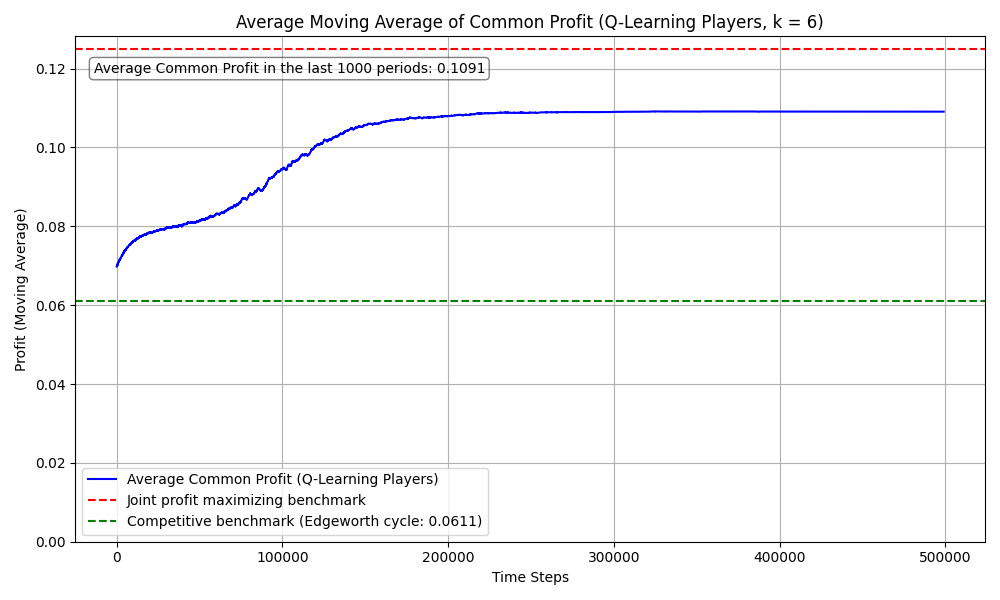
\includegraphics[width=\linewidth]{K=6.png}
        \caption{Q-learner vs Q-learner }
        \label{fig: K = 6}
    \end{minipage}
    \hfill
    \begin{minipage}{0.75\linewidth}
        \centering
        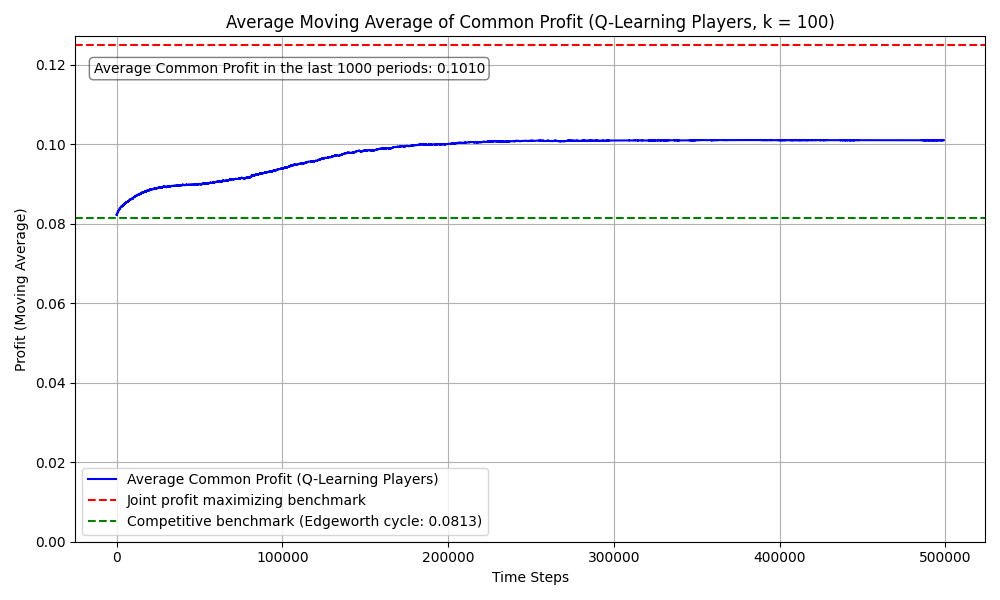
\includegraphics[width=\linewidth]{K=100.png} % Replace with your second image
        \caption{Q-learner vs Q-learner }
        \label{fig: K = 100}
    \end{minipage}
\end{figure}

\subsubsection{Random vs Random}
Figure \ref{fig: RANDOM K = 6} and \ref{fig: RANDOM K = 100} illustrate our simulation results for when two Random players played against each other when K was 6 and 100, respectively. Similar graphs for k values of 12, 24 and 48 can be found in the appendix, in figure \ref{fig:}, \ref{fig:} and \ref{fig: }. This was done by simply having each player sequentially pick a random price with equal probability when it was their turn. Unlike for the Q-learner game, the figures here finely illustrate that no learning is taking place as the plotting of the Average common profit (purple line) does not have any significant fluctuations from start to finish. By our measurements the random players do technically behave collusively, but still not nearly as much as the Q-learner. The random vs Random player figures illustrate finely how the Q-learner are learning and converging towards more collusive strategies.   

\begin{figure}[H]
    \centering
    \begin{minipage}{0.75\linewidth}
        \centering
        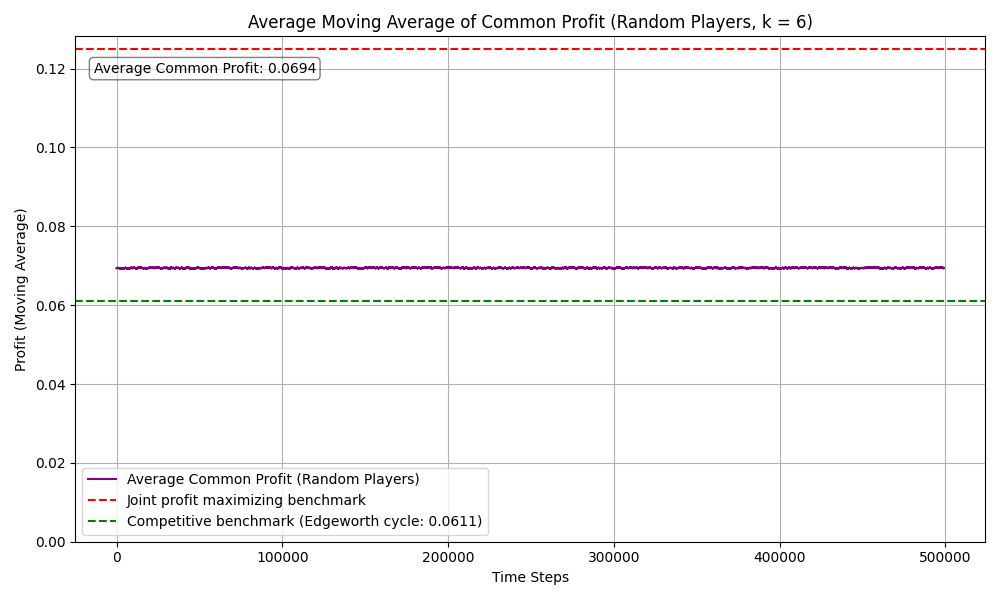
\includegraphics[width=\linewidth]{RANDOM PLAYER, K=6.png}
        \caption{Random players, k = 6 }
        \label{fig: RANDOM K = 6}
    \end{minipage}
    \hfill
    \begin{minipage}{0.75\linewidth}
        \centering
        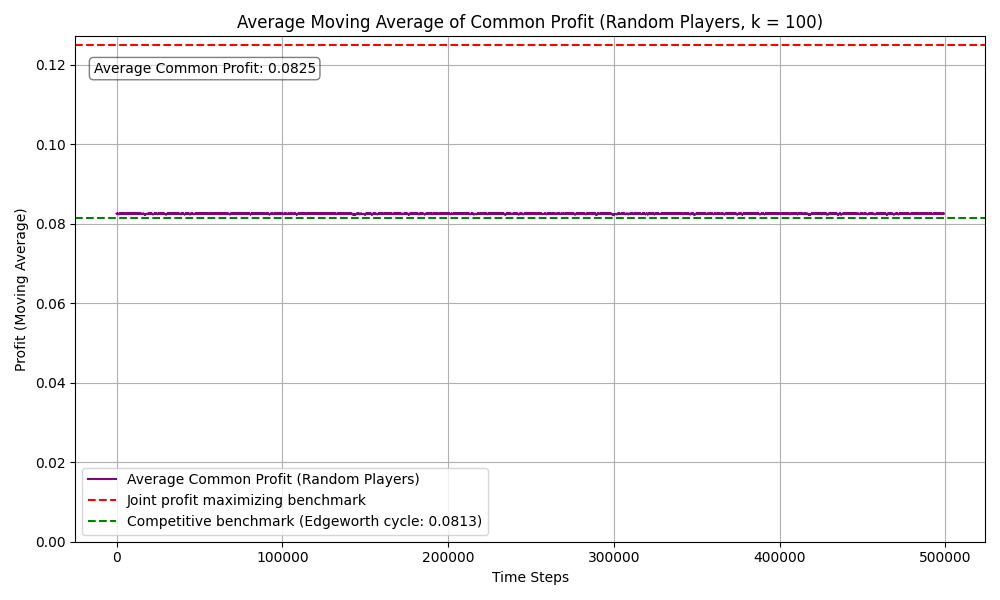
\includegraphics[width=\linewidth]{RANDOM PLAYER, K=100.png}
        \caption{Random players, k = 100}
        \label{fig: RANDOM K = 100}
    \end{minipage}
\end{figure}


\subsection{Level of Collusion for K values}
\label{Level of Collusion for K values}
\subsection{Convergence Analysis}
\label{Convergence Analysis}
\subsubsection{MOTHER GRAPH}
\subsubsection{In-depth look at cycles}
\label{In-depth look at cycles}


\section{Discussion}


\section{Conclusion}

\newpage 


\section{References}

\bibliographystyle{apalike}
\bibliography{references}


\section{Appendix}
\subsection{Q-learning collusion graphs}

\subsubsection{k = 12}
\begin{figure}[H]
    \centering
    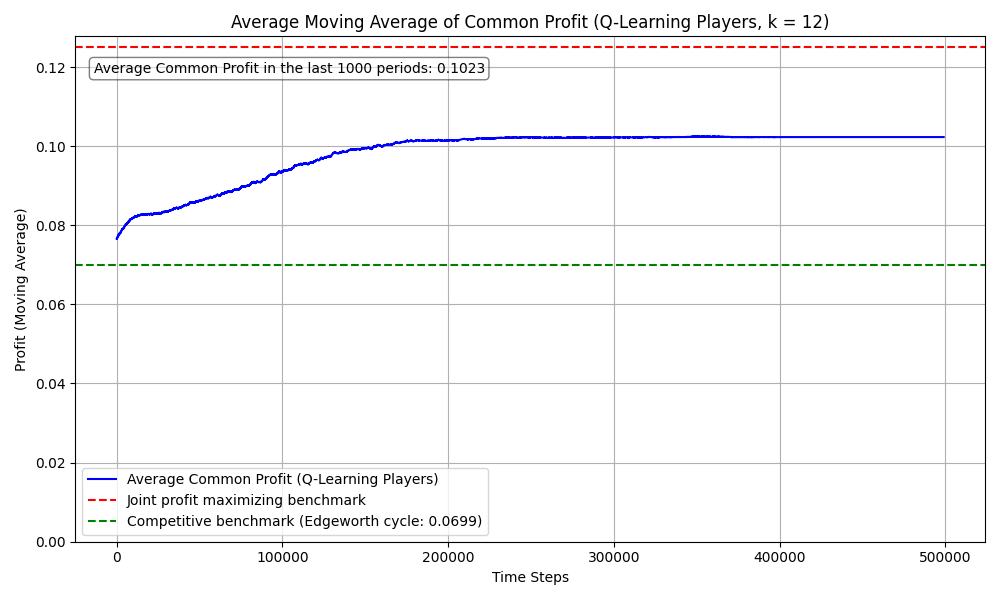
\includegraphics[scale = 0.45]{K=12.png}
    \caption{Q-learner vs Q-learner when k = 12}
    \label{fig: QlearnervQlearnerK=12}
\end{figure}

\subsubsection{k = 24}
\begin{figure}[H]
    \centering
    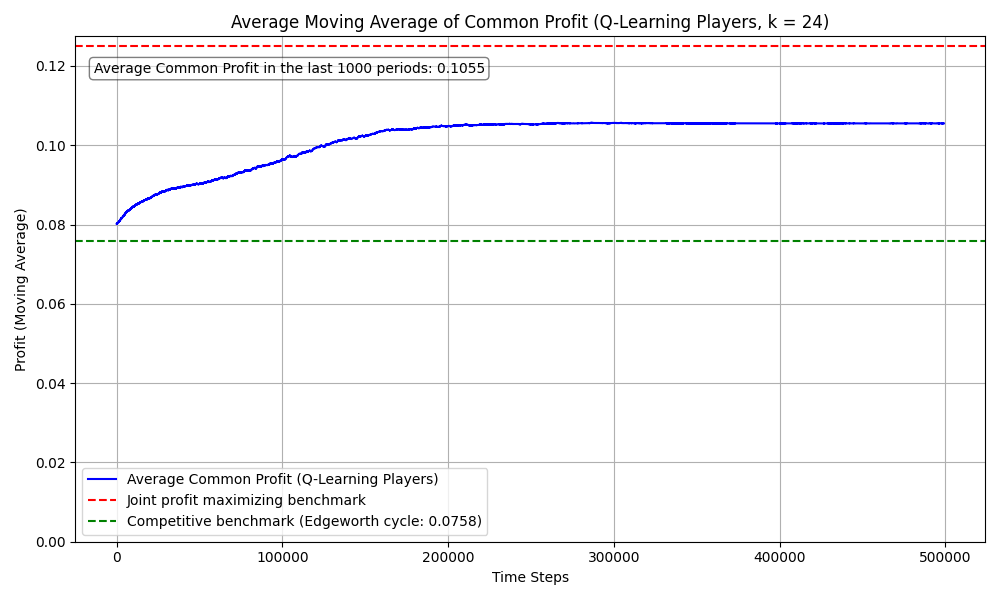
\includegraphics[scale = 0.45]{K=24.png}
    \caption{Q-learner vs Q-learner when k = 24}
    \label{fig: QlearnervQlearnerK=24}
\end{figure}

\subsubsection{k = 48}
\begin{figure}[H]
    \centering
    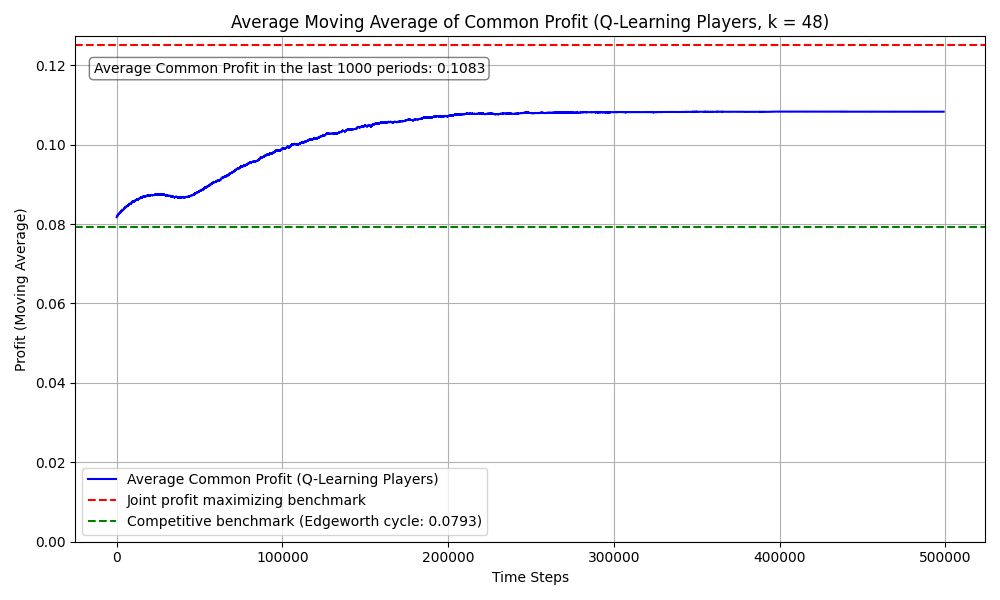
\includegraphics[scale = 0.45]{K=48.png}
    \caption{Q-learner vs Q-learner when k = 48}
    \label{fig: QlearnervQlearnerK=48}
\end{figure}


\end{document}
